\chapter{Introduction}

The fingerprint is the systematic compilation on a given device in order to identify it, singularize it and profile it. This data set practically allows, univocally, to identify that device and the person or group of people who may be using it. In general, devices such as mobile phones, tablets, laptops and desktop computers are used by a single person and therefore, we can assume that the data collected from a certain device belongs to a specific person. \par

Currently, web applications provide services completely free of charge in exchange for the data they collect from users. In most cases, this information is made profitable through marketing and advertising services that desire to sell a specific product or service. Therefore, these services need to profile the user in order to offer them a product that may be of their interest. Entities use these data compilation mechanisms with all devices that connect to their servers, in order to monitor the user and create a profile. \par

The best-known tracking technique is by cookies, which are stored on the device itself and then used to study the statistics of web application usage and to improve the user experience. It is common to find privacy clauses that allow the user to give or not consent to their use. Some browsers offer the possibility of disabling their use and some antivirus perform periodic deletions of the trace files, but most web applications do not allow access to their services, or all of them, if the user does not allow their use. Using fingerprint techniques allows that, in the case that the \textit{cookies} are deleted, the traceability on the user is not lost. Technologies such as JavaScript, Flash and Microsoft Silverlight, facilitate the implementation of methods to collect very specific information from the device, such as the screen size or the operating system version. The combination of these characteristics allows the user to be profiled and identified. \par

\section{Objetives}
 

The main objective of this project is to create a web application that allows the collection of data from a device, applying the different fingerprinting techniques, and to elaborate a profile based on them. Specifically, we have the following goals:
\begin{itemize}
    \item Create a scalable application, so that it can be further developed as required in the future.
    \item Research the variety of fingerprint methods and implement them.
    \item Store the collected information, from which will be profiled and saved in a database.
\end{itemize}

\section{Workplan}
For the development of the project, a plan has been established in such a way that the research, requirements analysis, implementation, testing and report phases are covered. \par
The figure~\ref{fig:diagramaGantten} shows the Gantt chart. After the deadlines were extended, subsequent tasks and their respective times were updated. The broken down tasks consist of:
\begin{itemize}
    \item \textbf{Research}: Information gathering about the various available techniques\cite{Huella} to obtain data from the devices. This includes certain pages that determine the browser's fingerprint.\cite{amiunique}.
    \item \textbf{Requirements analysis}: Assessment about which programming language and tools we are going to use for the development of the project.
    \item \textbf{Implementation}: Start up of the project. At this stage of development the web application would be implemented with its respective database.
    \item \textbf{Testing}: Functional verification and testing of the application and resolution of possible incidents.
    \item \textbf{Report}: Document reflecting the development and results of the project.
\end{itemize}
\begin{figure}[b]
    %\centering
    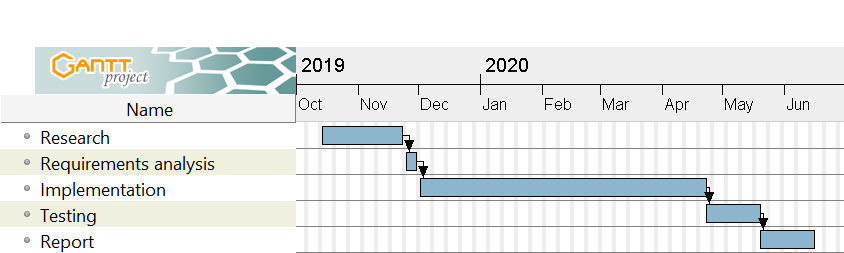
\includegraphics[width=1\textwidth, height=4cm]{Images/diagramaGantten.png}
    \caption{Gantt chart}
    \label{fig:diagramaGantten}
\end{figure}

\section{Content}
The document includes the following chapters:
\begin{itemize}
    \item \textbf{Preliminary}: Starting point and presentation of the different technologies and tools that have been explored.
    \item \textbf{Information sources}: Briefing of the main data sources used for fingerprinting.
    \item \textbf{Design and implementation}: Description on how the application works.
    \item \textbf{System use}: Brief demonstration where the use of the application is observed.
    \item \textbf{Individual contribution}: Detailed contribution of each member of the project.
    \item \textbf{Conclusions}: The obtained results are reasonably discussed.
\end{itemize}
